\subsection{Eigenschaften}

Wie schon erwähnt spezifizieren Klassen Eigenschaften, die alle ihre Instanzen besitzen sollen. Dabei werden im Zuge der Abstraktion zwischen Realwelt und Modell nur diejenigen Eigenschaften der zu modellierenden Realwelt-Objekte berücksichtigt, die für den Modellzweck relevant sind. In UML-Notation werden die Eigenschaften in Form von Attributen im Rechteck der jeweiligen Klasse verzeichnet. Dafür wird das Rechteck unterhalb des Klassennamens durch eine Linie horizontal geteilt.
\begin{wrapfigure}{o}[70pt]{0.6\textwidth}
	%\vspace{-10pt}
	\centering 
	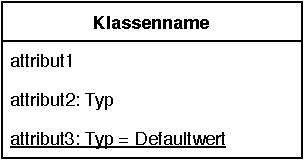
\includegraphics{../grafiken/Kapitel-3/Abb-3-7.pdf}
	\caption{Eine Klasse mit Attributen in UML-Darstellung}
	\label{fig:Abb-3-7}
	\vspace{-6pt}
\end{wrapfigure}
Abbildung~\ref{fig:Abb-3-7} zeigt drei gängige Varianten, wie Attribute innerhalb einer Klasse angegeben werden können.\footnote{Die UML lässt noch weitere Varianten zu.} Wir werden im weiteren Verlauf des Kurses sehen, dass für unterschiedliche Zwecke während des Softwareentwicklungsprozesses unterschiedlich stark detaillierte Klassendiagramme benötigt werden. So wird zum Beispiel in Domänenklassendiagrammen üblicherweise nur der Attributname angegeben, während Klassendiagramme, die auf die Implementierung ausgerichtet sind, die Informationen über Attributtypen und evtl. Vorgabewerte (default values) beinhalten müssen. Sofern Attributtypen in einer Klasse angegeben werden, muss es sich zudem nicht zwangsläufig um programmiersprachliche Datentypen handeln. Gerade in Klassendiagrammen, die für die Kommunikation mit Nicht-Programmierern gedacht sind, finden sich häufiger Angaben wie Euro oder Grad Celsius statt Integer oder Float.

Abbildung~\ref{fig:Abb-3-8} zeigt oben die Klasse \texttt{Auto}, die über die beiden Attribute \texttt{modell} und \texttt{farbe} zwei Eigenschaften von Auto-Objekten spezifiziert.
\begin{wrapfigure}{o}[70pt]{0.8\textwidth}
	%\vspace{-10pt}
	\centering 
	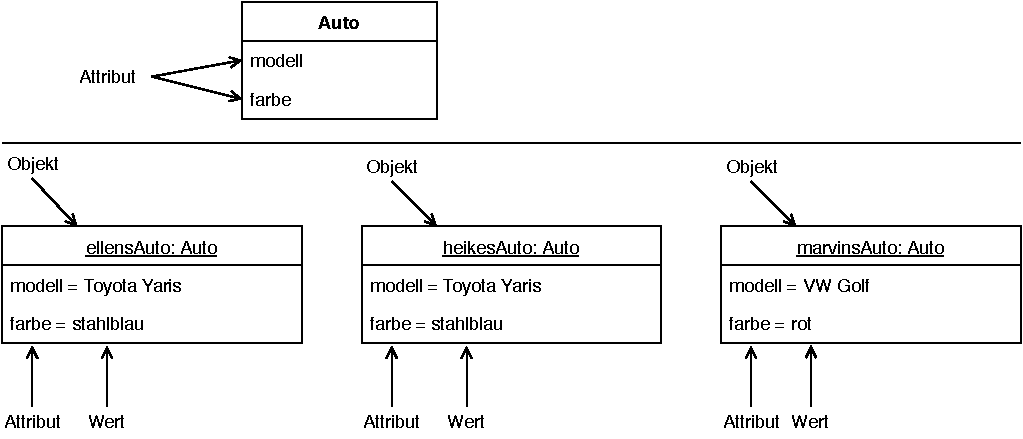
\includegraphics[scale=0.6]{../grafiken/Kapitel-3/Abb-3-8.pdf}
	\caption{Eine Klasse Auto und drei konkrete Instanzen der Klasse}
	\label{fig:Abb-3-8}
	\vspace{-6pt}
\end{wrapfigure}
Die Abbildung zeigt außerdem mit \texttt{ellensAuto}, \texttt{heikesAuto} und \texttt{marvinsAuto} drei konkrete Instanzen der Auto-Klasse, bei denen die Attribute \texttt{modell} und \texttt{farbe} mit konkreten Werten belegt sind. Attribute werden durch die Klasse definiert und sind für jede Instanz vorgegeben. Alle drei Auto-Objekte in Abbildung~\ref{fig:Abb-3-8} beinhalten daher die beiden Attribute \texttt{modell} und \texttt{farbe}. Ein Objekt kann zudem keine Attribute besitzen, die die Klasse nicht vorsieht. So kann zum Beispiel ein konkretes Auto-Objekt keine Angabe über das Baujahr des Autos beinhalten, solange die Klasse Auto ein solches Attribut nicht vorsieht, auch wenn das Realwelt-Auto, das durch das Auto-Objekt abgebildet wird, ein Baujahr besitzt. Die Wertebelegung der vorgegebenen Attribute ist dagegen objektspezifisch und auch veränderlich. So könnte für \texttt{marvinsAuto} die Wertebelegung des Attributs \texttt{farbe} von rot zu grün wechseln, wenn das Auto zum Beispiel neu lackiert wird. Die Änderung der Wertebelegung einer Instanz hat weder Auswirkungen auf ihre Klasse noch auf andere Instanzen derselben Klasse. Die aktuellen Wertebelegungen aller Attribute eines Objektes sowie seine bestehenden Verbindungen zu anderen Objekten (s.u.) bestimmen den so genannten Zustand des Objektes. Daraus ergibt sich, dass sich der Zustand eines Objektes ändert, wenn sich mindestens eine Wertebelegung seiner Attribute ändert. Die Identität eines Objektes ändert sich dagegen niemals. Sie besteht vom Zeitpunkt der Erzeugung bis zur Zerstörung des Objektes, unabhängig davon, wie häufig sich der Zustand des Objektes verändert hat.

Die beiden Auto-Instanzen \texttt{ellensAuto} und \texttt{heikesAuto} stimmen in den Wertebelegungen der Attribute \texttt{modell} und \texttt{farbe} überein. Man bezeichnet Objekte (derselben Klasse), die denselben Zustand aufweisen als zustandsgleich. Zustandsgleiche Objekte sind weiterhin Objekte mit unterschiedlicher Identität! Von der Zustandsgleichheit zu unterscheiden, ist die so genannte referentielle Gleichheit. Referentielle Gleichheit liegt vor, wenn sich hinter zwei unterschiedlichen Objektnamen das identische Objekt verbirgt, es sich also nur um zwei Referenzen auf dasselbe Objekt handelt. Zum Beispiel könnte die Realwelt-Person Henrike Meyer außer über ihren Namen auch über ihre Aliase Bürgermeisterin oder 1.~Vorsitzende des Elternrates bezeichnet werden. Die drei modellierten Objekte zeigen dann nur unterschiedliche Ausschnitte desselben Objektes, nämlich desjenigen Objektes, das die Realwelt-Person Henrike Meyer, die gleichzeitig Bürgermeisterin und 1.~Vorsitzende des Elternrates der Schule ihres Kindes ist, abbildet.

Manche Eigenschaften von Realwelt-Objekten, wie zum Beispiel der Modelltyp eines Autos, ändern sich nicht. Bei der Abbildung einer Eigenschaft auf ein System-Objekt möchte man eine solche Unveränderlichkeit vielleicht auch vorsehen. 
\begin{wrapfigure}{o}[70pt]{0.6\textwidth}
	%\vspace{-10pt}
	\centering 
	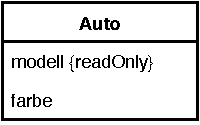
\includegraphics{../grafiken/Kapitel-3/Abb-3-9.pdf}
	\caption{Eine Klasse Auto mit einem unveränderlichen Attribut \texttt{modell} und einem veränderlichen Attribut \texttt{farbe}}
	\label{fig:Abb-3-9}
	\vspace{-6pt}
\end{wrapfigure}
Die UML sieht dafür die Angabe des ergänzenden Merkmals \{readOnly\} vor, die in der Klasse hinter dem Attribut notiert wird, aus Übersichtlichkeitsgründen aber nicht in den einzelnen Objekten (Abbildung~\ref{fig:Abb-3-9}). Die Klasse Auto (und das umgebende Programm) muss dann natürlich später auch so implementiert werden, dass sichergestellt ist, dass jede Auto-Instanz einen Attributwert für \texttt{modell} enthält, dieser Wert aber während der Lebenszeit der Instanz nicht verändert werden kann. In objektorientierten Programmiersprachen ist der Einsatz von Konstanten eine Möglichkeit, die Unveränderlichkeit von Attributwerten zu gewährleisten. Die Angabe von ergänzenden Merkmalen in geschweiften Klammern sieht die UML für verschiedene Zwecke vor und zwar nicht nur in Zusammenhang mit Attributen sondern auch mit Operationen und Beziehungen zwischen Elementen. Wir werden im Laufe des Kurses noch einige von der UML vordefinierte ergänzende Merkmale kennenlernen. Die UML erlaubt darüber hinaus auch benutzerdefinierte ergänzende Merkmale. Im letzteren Fall muss der Ersteller des UML-Diagramms allerdings sicherstellen, dass seine Zielgruppe die Bedeutung der modellierten Ergänzungen versteht.

Bisher haben wir Attribute betrachtet, die zwar durch die Klasse definiert werden, für die aber jede Instanz der Klasse ihre eigenen Wertebelegungen hat. Das Klassenkonzept der Objektorientierung sieht neben solchen Attributen, die auch als Instanzattribute bezeichnet werden, noch eine andere Art von Attributen vor, die so genannten Klassenattribute. 
Ein Klassenattribut ist ein Attribut, das in der Klasse verortet ist und dessen Wert von allen Instanzen der Klasse geteilt wird. Im Unterschied zu Instanzattributen besitzt also nicht jede Instanz eine eigene Wertebelegung für dieses Attribut, sondern es existiert nur ein gemeinsamer Wert. Jede Instanz kann auf das Attribut zugreifen, den Wert des Attributes auslesen und sofern es veränderlich ist, auch den Wert des Attributes ändern. Letzteres sollte bei der konkreten Implementierung geeignet gesteuert werden, da eine durch eine Instanz vorgenommene veränderte Wertebelegung eines Klassenattributes sich auf alle Instanzen der Klasse auswirkt. Klassenattribute verwendet man für die Abbildung von Eigenschaften, die relevant für die inhaltliche Modellierung einer konkreten Klasse sind, sich aber nicht den einzelnen Instanzen der Klasse zuordnen lassen. Ein Klassenattribut existiert auch dann, wenn (noch) keine Instanz der Klasse erzeugt wurde. \begin{wrapfigure}{o}[70pt]{0.8\textwidth}
	%\vspace{-10pt}
	\centering
	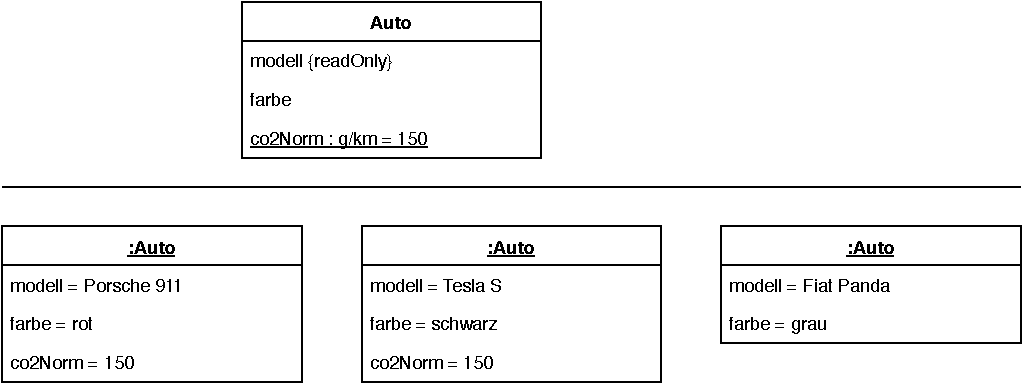
\includegraphics[scale=0.6]{../grafiken/Kapitel-3/Abb-3-10.pdf}
	\caption{Eine Klasse \texttt{Auto} mit Instanzattributen \texttt{modell} und \texttt{farbe} und dem Klassenattribut \texttt{co2Norm} (oben) sowie drei anonyme Instanzen der Klasse Auto (unten)}
	\label{fig:Abb-3-10}
	\vspace{-6pt}
\end{wrapfigure}
Ein Klassenattribut in unserem Autobeispiel-Kontext könnte \texttt{co2Norm} sein, wenn wir idealisiert annehmen, dass für alle Automodelle eine einheitliche CO$_2$-Abgasnorm gilt (Abb.~\ref{fig:Abb-3-10}). Klassenattribute werden in der UML-Darstellung der Klasse unterstrichen. In der Darstellung der Instanzen wird ein Klassenattribut identisch zu den Instanzattributen dargestellt. Häufig werden Klassenattribute aber aus Redundanzgründen (da jede Instanz denselben Wert hat) gar nicht in der Darstellung der Instanzen aufgeführt. Die UML erlaubt es, dass die Angabe der Attribute einer Instanz – nicht nur bezogen auf Klassenattribute sondern auch auf die Instanzattribute – unvollständig ist, weil zum Beispiel nur diejenigen Attribute aufgeführt werden sollen, bei denen noch Diskussionsbedarf besteht.